\documentclass[11pt]{article}

%%%%%%%%%%%%%%Include Packages%%%%%%%%%%%%%%%%%%%%%%%%%%
\usepackage{xcolor}
\usepackage{mathtools}
\usepackage[a4paper, total={6in, 8in}, margin=1.25in]{geometry}
\usepackage{amsmath}
\usepackage{amssymb}
\usepackage{paralist}
\usepackage{rsfso}
\usepackage{amsthm}
\usepackage{wasysym}
\usepackage[inline]{enumitem}   
\usepackage{hyperref}
\usepackage{tocloft}
\usepackage{titlesec}
\usepackage{colortbl}
\usepackage{wrapfig}
%%%%%%%%%%%%%%%%%%%%%%%%%%%%%%%%%%%%%%%%%%%%%%%%%%%%%%%%



\begin{document}
\Large \noindent \textbf{Physics 5A Discussion (Week 1)}\\
\normalsize
Department of Physics and Astronomy, UCLA\\
\noindent\rule{8cm}{0.4pt}\\

\begin{wrapfigure}[8]{r}{0.4\textwidth}
  \begin{center}
  \vspace{-25pt}
    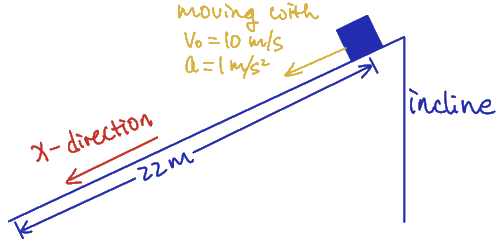
\includegraphics[width=0.45\textwidth]{incline}
  \end{center}
\end{wrapfigure}

\noindent\textit{Example}:
A box is sliding down from an incline (see figure). The acceleration of the box in the $x$-direction is $1$ m/s$^2$, and the initial velocity of the box in the $x$-direction is $10$ m/s. The incline is $22$ meters long. Find the time it takes to reach the bottom of the incline. \\

Since we know the initial velocity $v_0 = 10$ m/s, the acceleration of the box $a = 1$ m/s$^2$, the initial position $x_0 = 0$ m, and the final position $x_{\text{f}} = 22$ m. We can apply the kinematic equation directly, 
\begin{align*}
22 = x_{\text{f}} = \frac{1}{2} a t^2 + v_0 t + x_0 = \frac{1}{2}t^2 + 10 t + 0\,.
\end{align*}
Then we use the quadratic formula (for the polynomial $0 = at^2 + bt + c$) to find $t$, 
\begin{align*}
t = \frac{-b \pm \sqrt{b^2 -4ac}}{2a} = \frac{-10 \pm \sqrt{100 + 44}}{1} = 2\,.
\end{align*}
So it takes $2$ \underline{seconds} for it to reach the bottom of the incline. You probably have noticed that $t = -22$ seconds is also a solution due to the $\pm$ signs in the quadratic formula. Why can we just ignore that $t=-22$ seconds solution?\\

\begin{center}
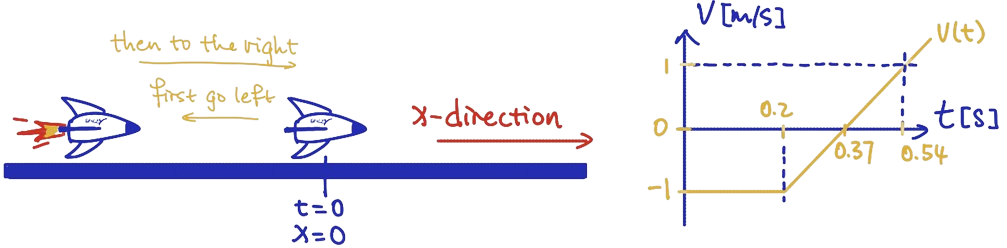
\includegraphics[scale=0.41]{rocket1}
\end{center}
\noindent \textbf{Problem 1}: A rocket is mounted on a track shown in the figure. The rocket initially has a speed moving to the left, then after a while the boost on the rocket is switched on, providing a constant acceleration to the right. Jinyan has obtained a velocity vs. time graph for the rocket as shown, and he asks you to draw the position vs. time, and acceleration vs. time graph for the rocket (You can assume that the position of the rocket at $t = 0$ s is $x =0$ m). 

\newpage
\begin{center}
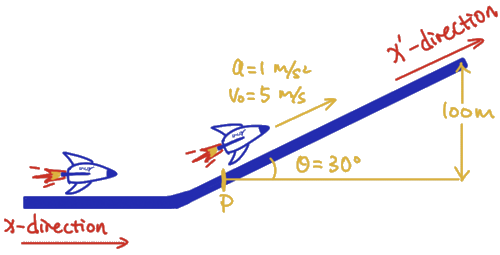
\includegraphics[scale=0.52]{rocket2}
\end{center}
\noindent \textbf{Problem 2}: After accelerating to the right for a few seconds, the rocket moves onto a ramp at an angle of $\theta = 30^\circ$. When it reaches point $P$ as shown, it has a velocity $v_0 = 5$ m/s in the $x'$-direction, but its acceleration in the $x'$-direction is down to $1$ m/s$^2$ due to gravity. How long does it take for the rocket to reach a height of $h = 100 $ m? \\

\noindent(\textit{Hint: How far does the rocket need to travel in the $x'$-direction to reach $h=100$ m?})
\newline\newline\newline
\newline\newline\newline
\newline\newline\newline
\newline\newline\newline
\newline\newline\newline
\newline\newline\newline
\noindent \textbf{Problem 3}: How far has the rocket traveled in the horizontal direction ($x$-direction) when it reaches $h = 100$ m. 



\end{document}


